\chapter{Dílčí části výukové sady}
Výuková sada je složená ze čtyř navzájem na sebe navazujících částí.
\fxnote[inline=true]{\textcolor{mygreen}{Sem ještě něco dopíšu, jen zatím nevím co...}}

\section{Výuková videa}
\fxnote[inline=true]{\textcolor{mygreen}{Sem ještě něco dopíšu, jen zatím nevím co...}}

\subsection{Formát a struktura výukových videí}
Ještě před tím, než jsem začal vytvářet jednotlivá videa jsem si musel odpovědět na několik důležitých otázek:
\begin{itemize}[topsep=0pt]
    \setlength\itemsep{0em}
    \item Jak budou videa koncipována? Bude se jednat o krátká videa zaměřená na jeden konkrétní prvek, nebo budou delší a zaměřená na širší problematiku?
    \item Kam budu hotová videa umisťovat?
    \item Jak budou videa vypadat po grafické i technické stránce?
\end{itemize}

Ve snaze najít odpověď na první z nich jsem se zamyslel, jakým způsobem sám vyhledávám informace.
Pokud potřebuji získat odpověď na konkrétní otázku v dlouhém textu, mám možnost využít textového vyhledávání. 
U videa ale žádná klávesová zkratka \It{Ctrl+F} zatím neexistuje -- musel bych tedy pomalu přeskakovat, až bych našel onu hledanou část.
Odpověď byla proto jasná -- krátká videa zaměřená na konkrétní prvek.

S druhou otázkou jsem si lámal hlavu o chvíli déle.
Na začátku jsem uvažoval nad umisťováním videí přímo na vlastní server, odkud by bylo možné je streamovat.
Nebyl bych vázaný limitací žádné služby a pokud by mi nějaká funkcionalita chyběla, mohl bych si ji snadno vyrobit.
Následně jsem si ale uvědomil, že tato varianta by konečnému divákovi nepřinesla žádný užitek.
V závěru jsem se rozhodl využít službu YouTube.
Její výhody pro koncového uživatele jsou jasné -- jedná se o velkou platformu, kterou dnes zná již téměř každý.
Pro studenty by tedy nebyl žádný problém s orientací, nebo dostupností obsahu (YouTube využívá vlastní CDN\footnote{Content delivery network, globální síť serverů určených pro distribuci obsahu}, díky které je zajištěná téměř stoprocentní dostupnost).

Posledním bodem bylo zvážení grafického designu a technické stránky.
Design sám o sobě prošel jistou proměnou, nicméně jsem se již od začátku snažil o to, aby videa vypadala moderně a čistě.
Po technické stránce jsem se rozhodl držet rozlišení 1920x1080 při 60 snímcích za vteřinu a hlasitosti zvukové stopy normalizované na -14 LUFS, což je standardní hlasitost pro videa nahrávaná na YouTube.
Těchto parametrů se od vydání prvního videa držím, aby byla všechna co možná nejjednotnější.

Mimo to bylo nutné připravit strukturu videí.
Vzhledem k tomu, že mají co nejstručněji a nejsrozumitelněji představit optimální řešení daného problému, rozhodl jsem se držet pouze třech důležitých bodů:
\begin{itemize}[topsep=0pt]
    \setlength\itemsep{0em}
    \item Úvod videa,
    \item potřebné hodnoty a parametry,
    \item samotný postup tvorby daného prvku.
\end{itemize}
V úvodu je v krátkosti popsáno zaměření videa a smysl daného prvku, popř. postupu.
U videí zaměřených na modelování následuje výčet potřebných hodnot a parametrů, které jsou zapotřebí.
Nakonec následuje názorná ukázka samotného postupu.

\subsection{Podkresová hudba}
Podstatné zlepšení dojmu z videí nastalo ve chvíli, kdy jsem začal do podkresu videa přidávat hudbu.
V samotných začátcích jsem čerpal skladby z platformy ncs.io, která poskytuje skladby k volnému užití za předpokladu uvedení autora a zdroje.
Postupně jsem ale došel k závěru, že skladby použité u některých původních videí nejsou vzhledem k edukativní povaze obsahu příliš vhodné a rozhodl se styl volené hudby změnit. 
Změnil jsem i zdroj hudby a začal čerpat z placené služby Artlist.io umožňující licencování obrovského množství hudby mnoha různých žánrů.

Při volbě skladby do podkresu se snažím volit žánry, které nebudou působit rušivě, příliš vážně, nebo naopak infantilně.
Hlasitost je vždy regulována dostatečně na to, aby byl komentář ve videu dobře srozumitelný a hudba do něj příliš nezasahovala.

\subsection{Náhledové obrázky}
V případě videí P3D mají náhledové obrázky smysl hlavně z hlediska orientace.
Snažil jem se proto, aby měly všechny jednotné rozložení a design a lišily se pouze částečně obsahem a barvami.
\begin{figure}[htbp]
    \centering
    \begin{minipage}[b]{0.45\textwidth}
        \centering
        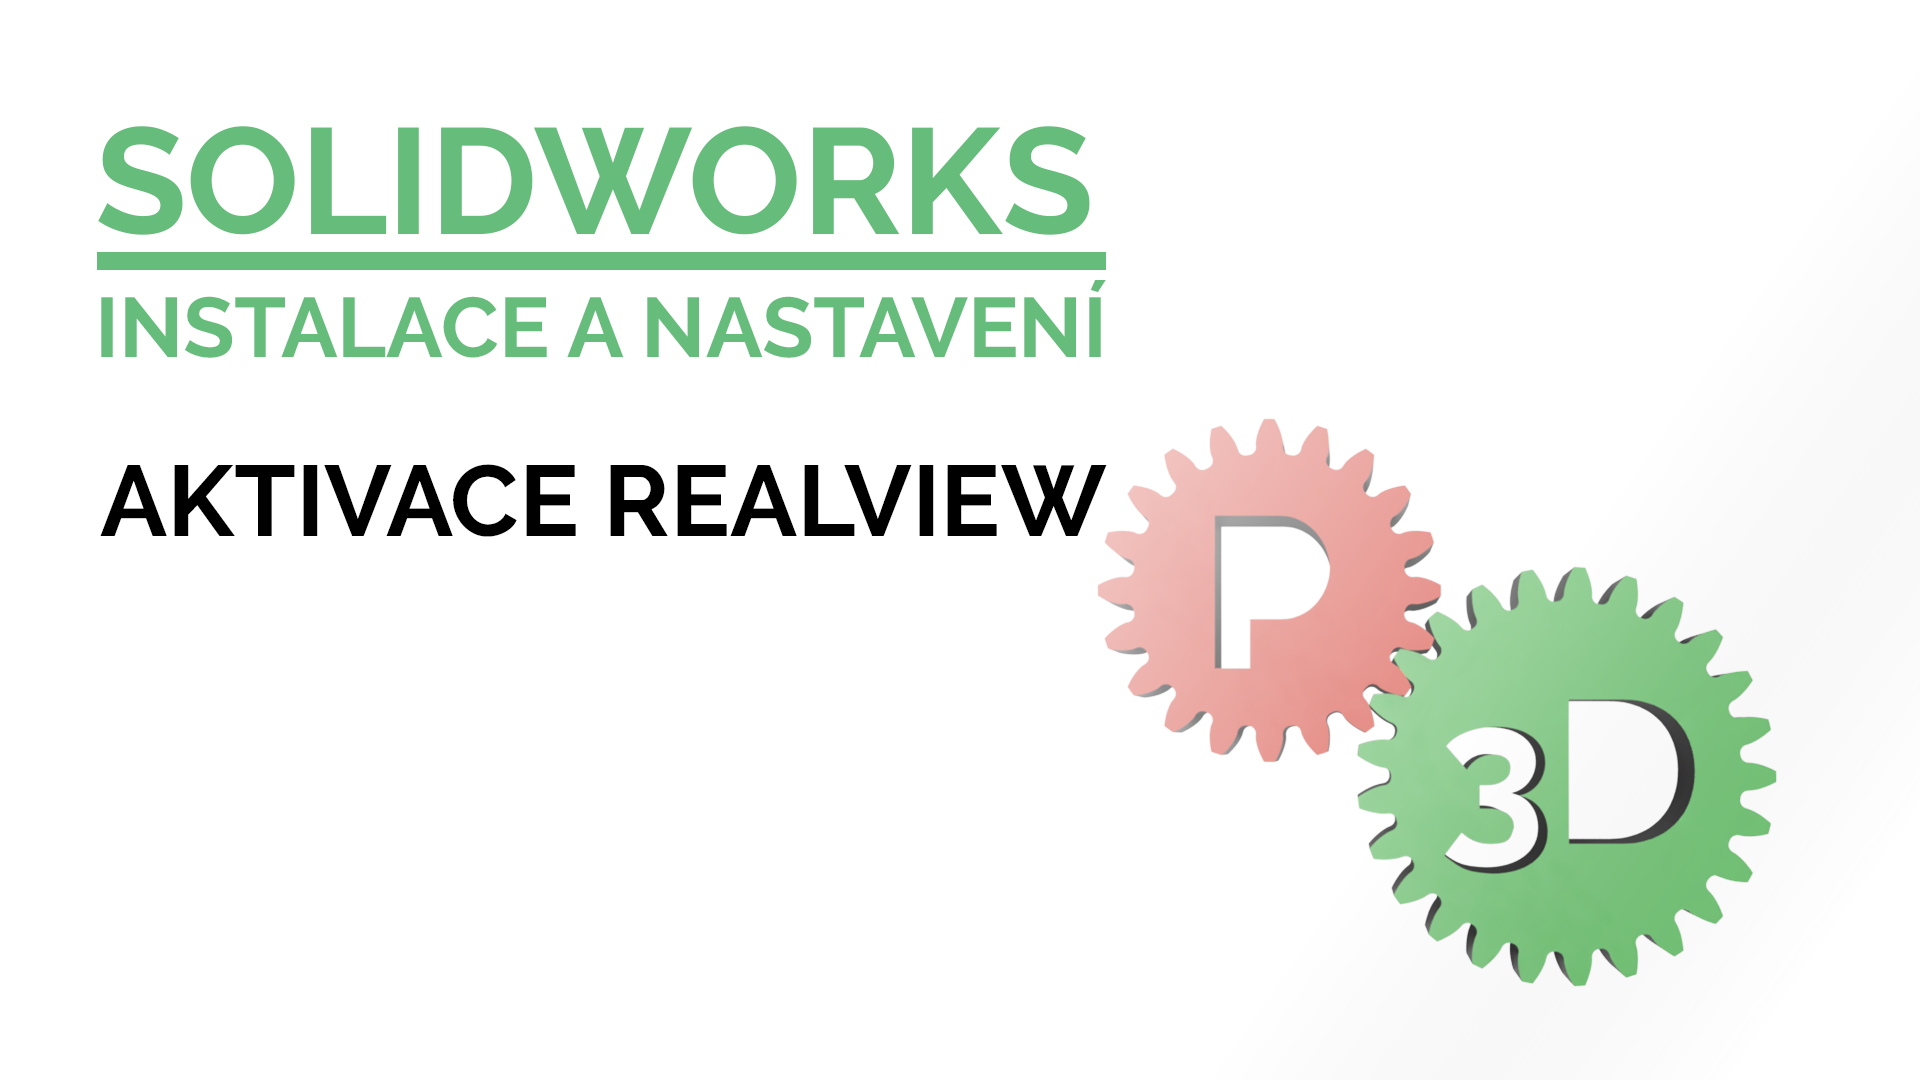
\includegraphics[width=0.8\textwidth]{img/020/aktivace-realview-thumbnail.png}
        \caption{Instalace a nastavení}
        \label{fig:thumb1}
    \end{minipage}
    \qquad
    \begin{minipage}[b]{0.45\textwidth}
        \centering
        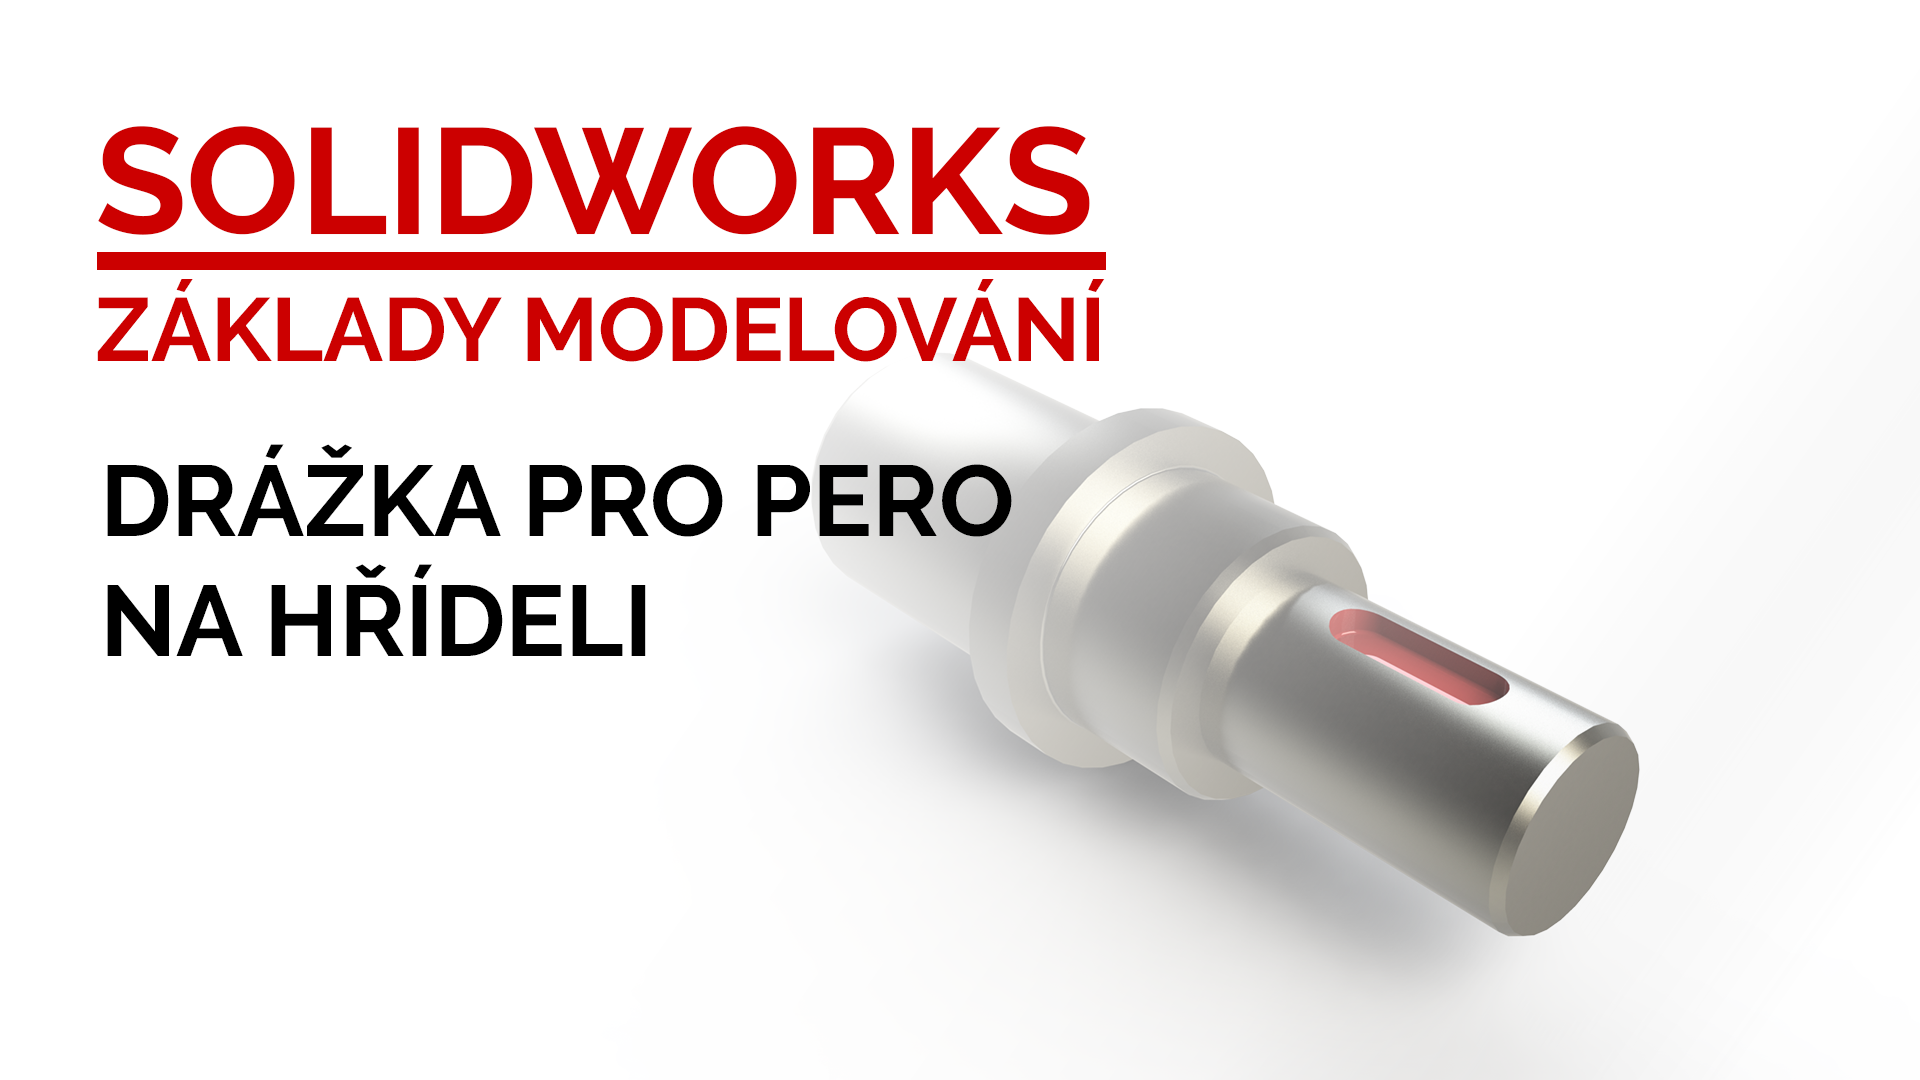
\includegraphics[width=0.8\textwidth]{img/020/perodr-hr-thumbnail.png}
        \caption{Modelování}
        \label{fig:thumb2}
    \end{minipage}
\end{figure}

\begin{figure}[htbp]
    \centering
    \begin{minipage}[b]{0.45\textwidth}
        \centering
        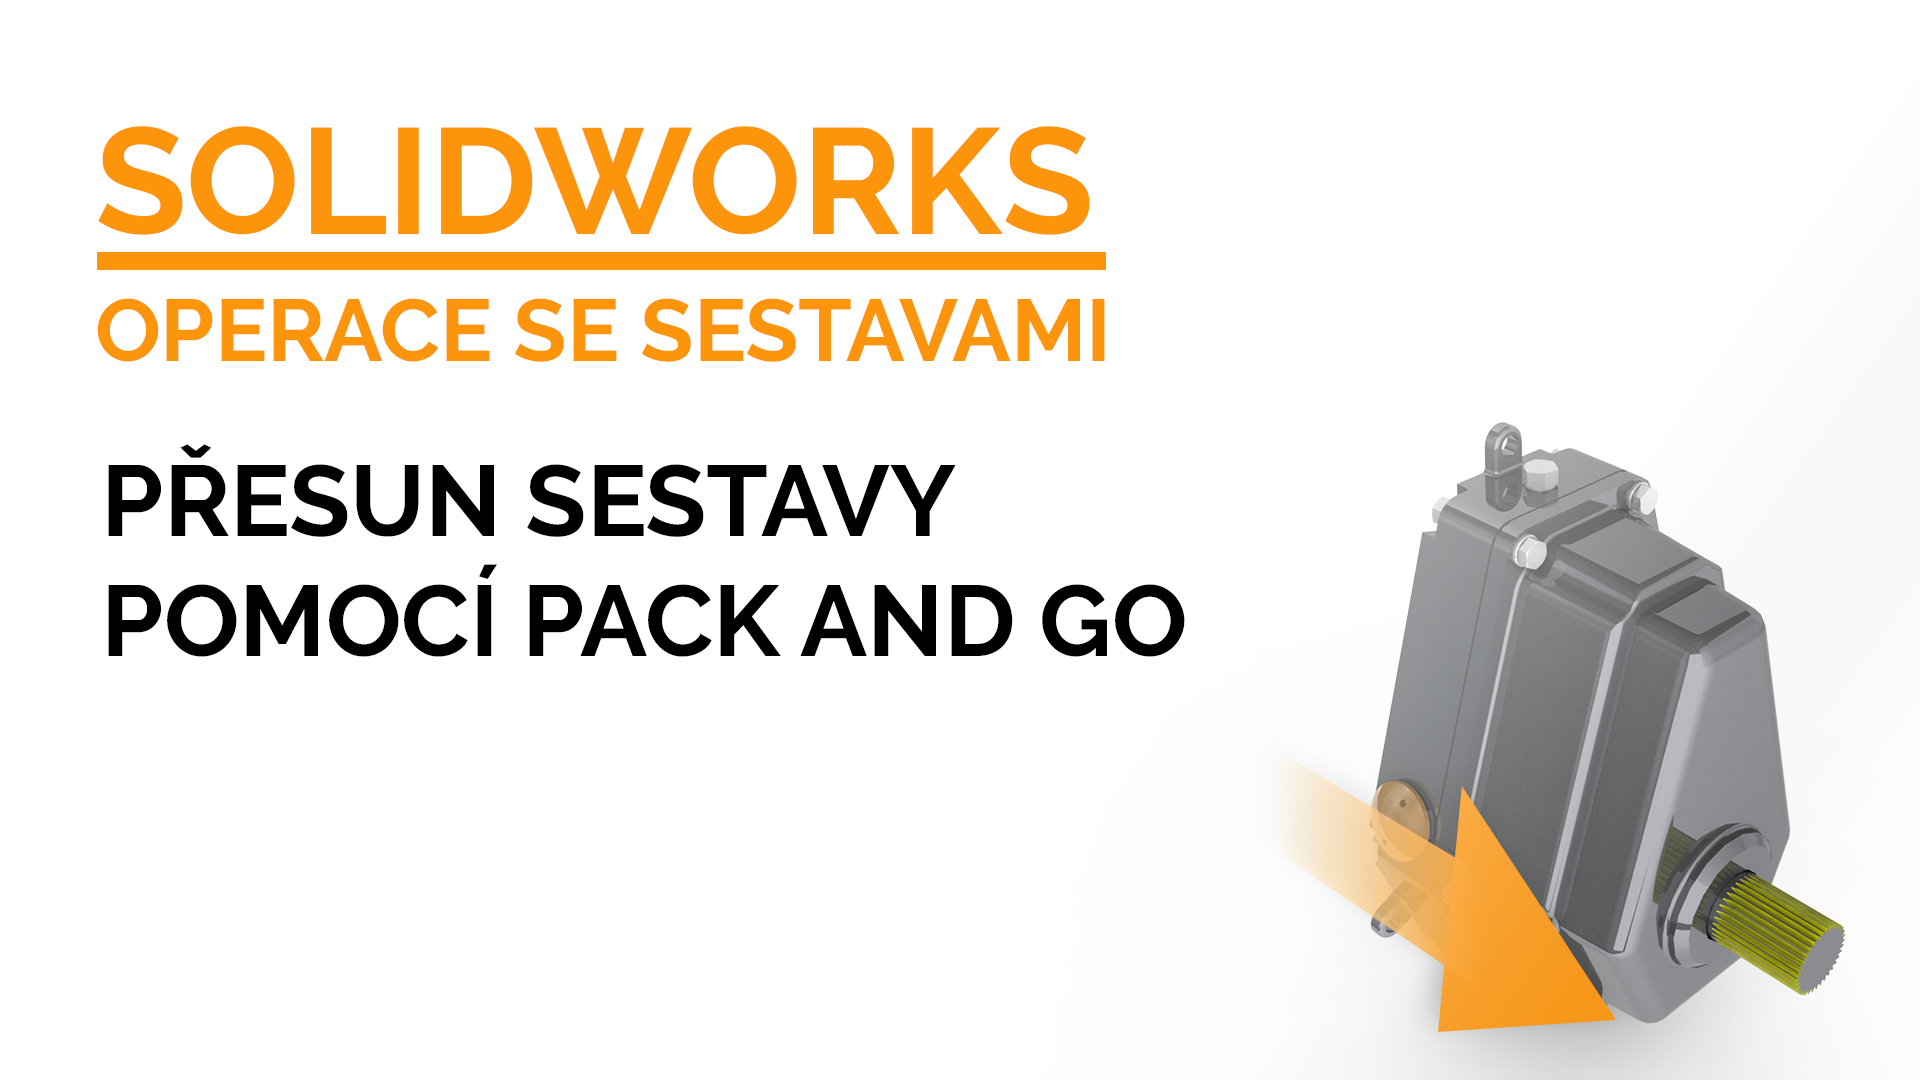
\includegraphics[width=0.8\textwidth]{img/020/pack-and-go-thumbnail.png}
        \caption{Sestavy}
        \label{fig:thumb3}
    \end{minipage}
    \qquad
    \begin{minipage}[b]{0.45\textwidth}
        \centering
        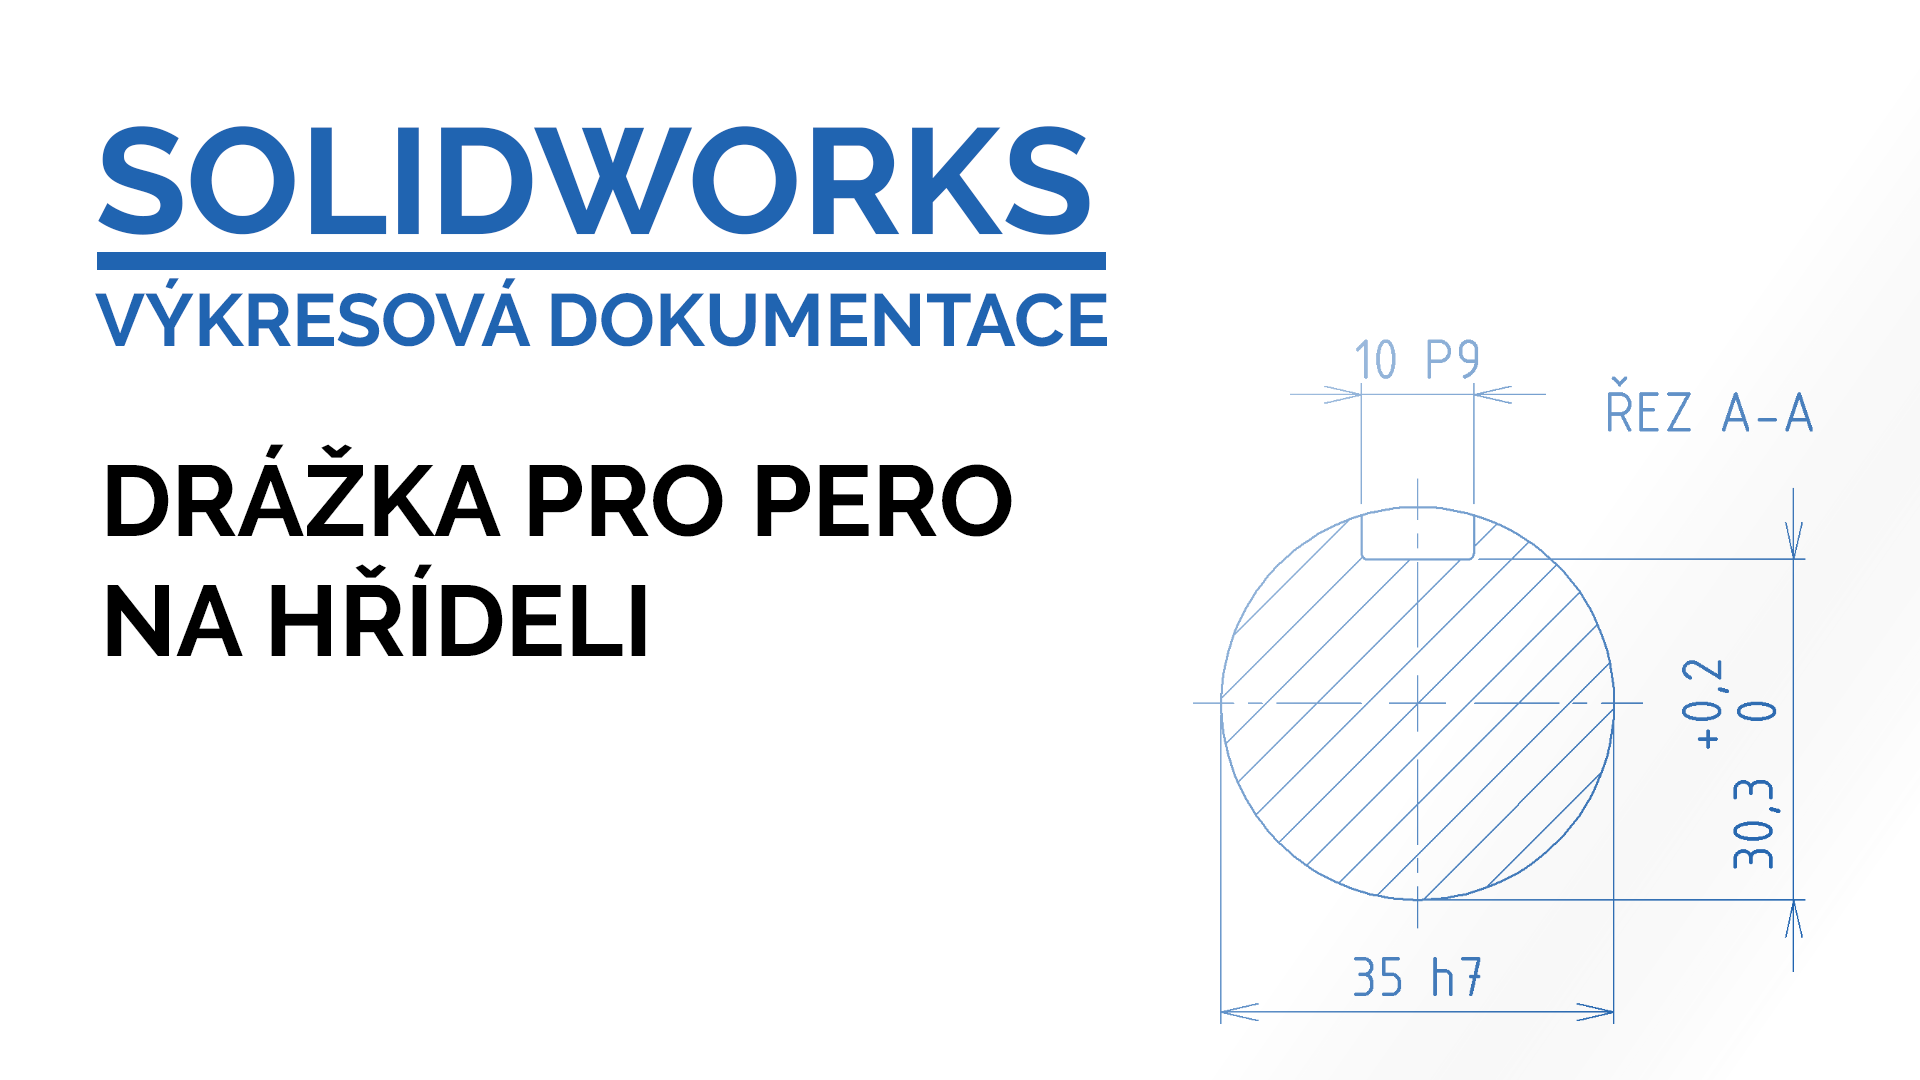
\includegraphics[width=0.8\textwidth]{img/020/dwg-perodr-hr-thumbnail.png}
        \caption{Výkresová dokumentace}
        \label{fig:thumb4}
    \end{minipage}
\end{figure}

Jak můžete vidět na jednotlivých náhledech \ref{fig:thumb1}, \ref{fig:thumb2}, \ref{fig:thumb3} a \ref{fig:thumb4}, každý z nich má v levém horním rohu umístěný nadpis s názvem série (resp. zaměřením), pod kterým se nachází konkrétní téma daného videa.
Na pravé polovině je v pozadí náhled doplněn obrázkem ilustrujícím dané téma (například hřídel s drážkou pro pero).

Díky tomuto systému je studentovi již ve chvíli, kdy vidí náhled jasné téma daného videa, což podstatně usnadňuje orientaci.
Zaměření videí jsou zároveň barevně odlišena, což umožňuje ještě rychlejší navigaci.
Při volbě barev jsem se snažil, aby nebylo možné je snadno zaměnit a byly vůči sobě dostatečně kontrastní.
Zvolené barvy mají za cíl od sebe témata barevně odlišit, nicméně nemají žádnou spojitost s konkrétními prvky, nebo funkcemi v SolidWorks.

\section{Tištěné materiály s otázkami a úkoly}
Samotná videa dokáží samostatně fungovat jako vzdělávací materiál, nicméně ne všem studentům může tato forma vyhovovat.
Proto jsem pro každé z videí vytvořil i psanou verzi vhodnou pro použití v prezenční výuce v případě, že není možnost třídě video promítnout, nebo je žádoucí, aby studenti pracovali samostatně.
\begin{figure}[htbp]
    \centering
    \begin{minipage}[b]{0.45\textwidth}
        \centering
        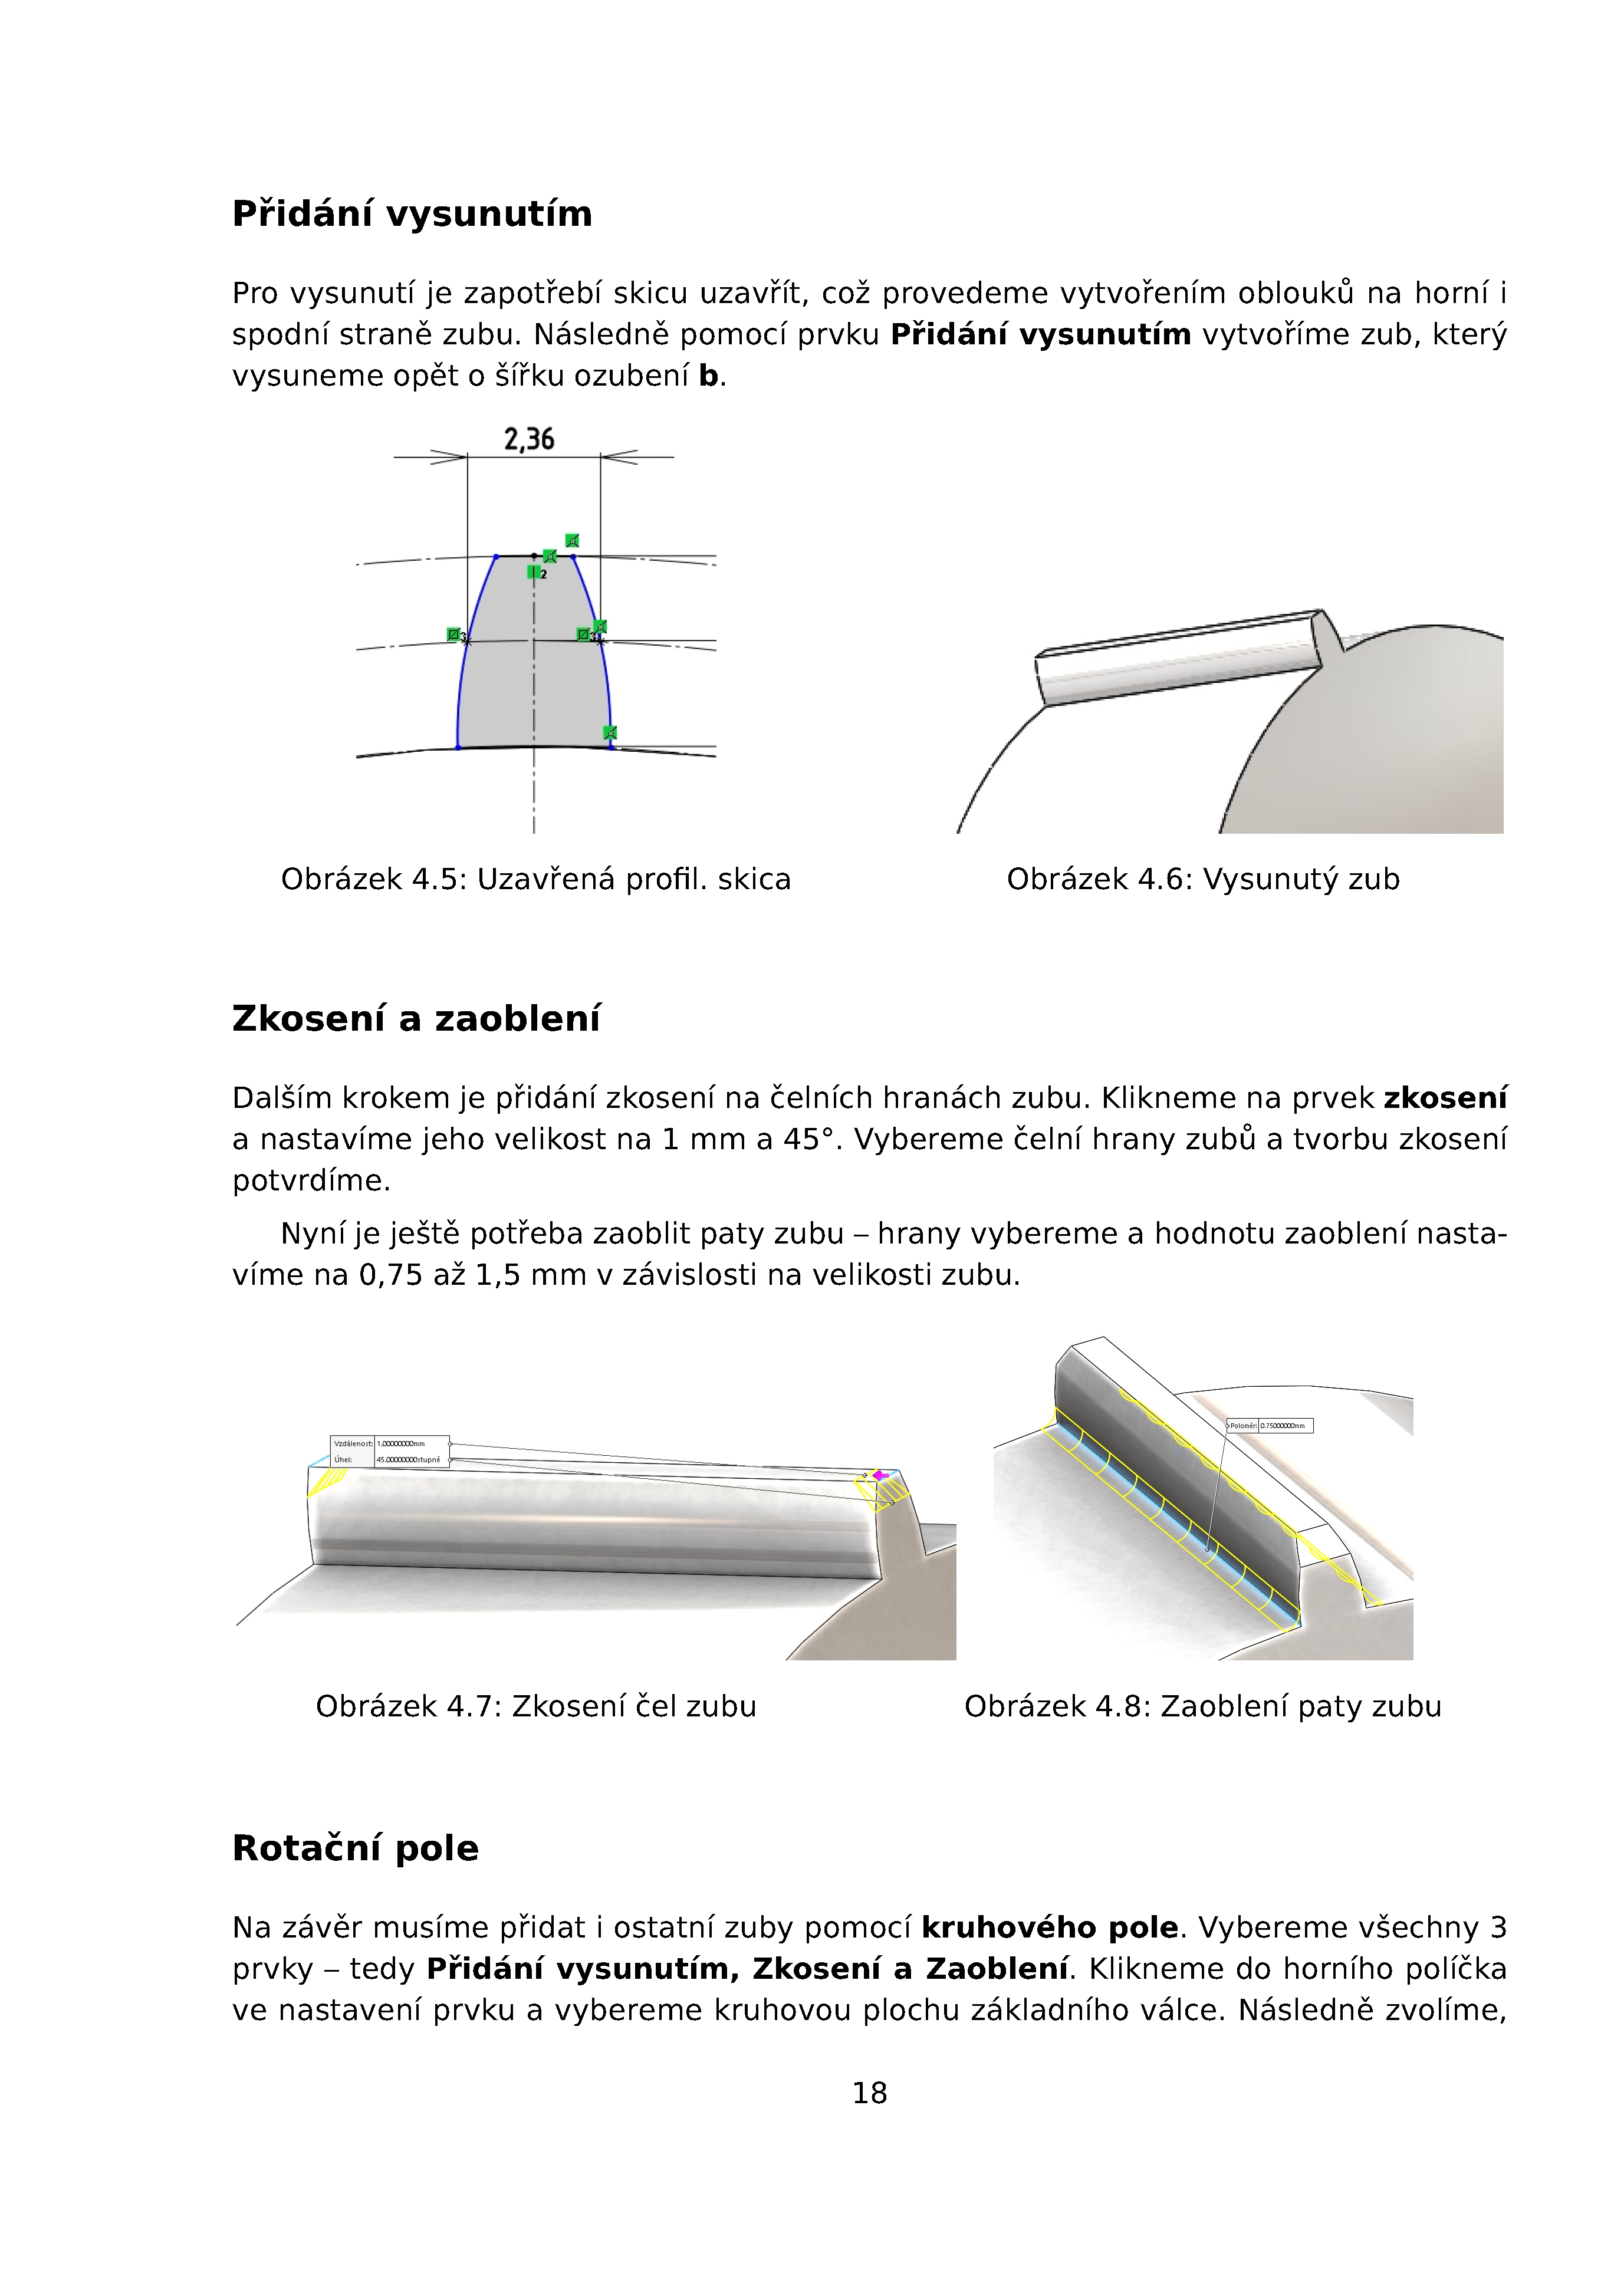
\includegraphics[width=0.8\textwidth]{img/020/guide1.png}
        \caption{Tištěné materiály}
        \label{fig:thumb3}
    \end{minipage}
    \qquad
    \begin{minipage}[b]{0.45\textwidth}
        \centering
        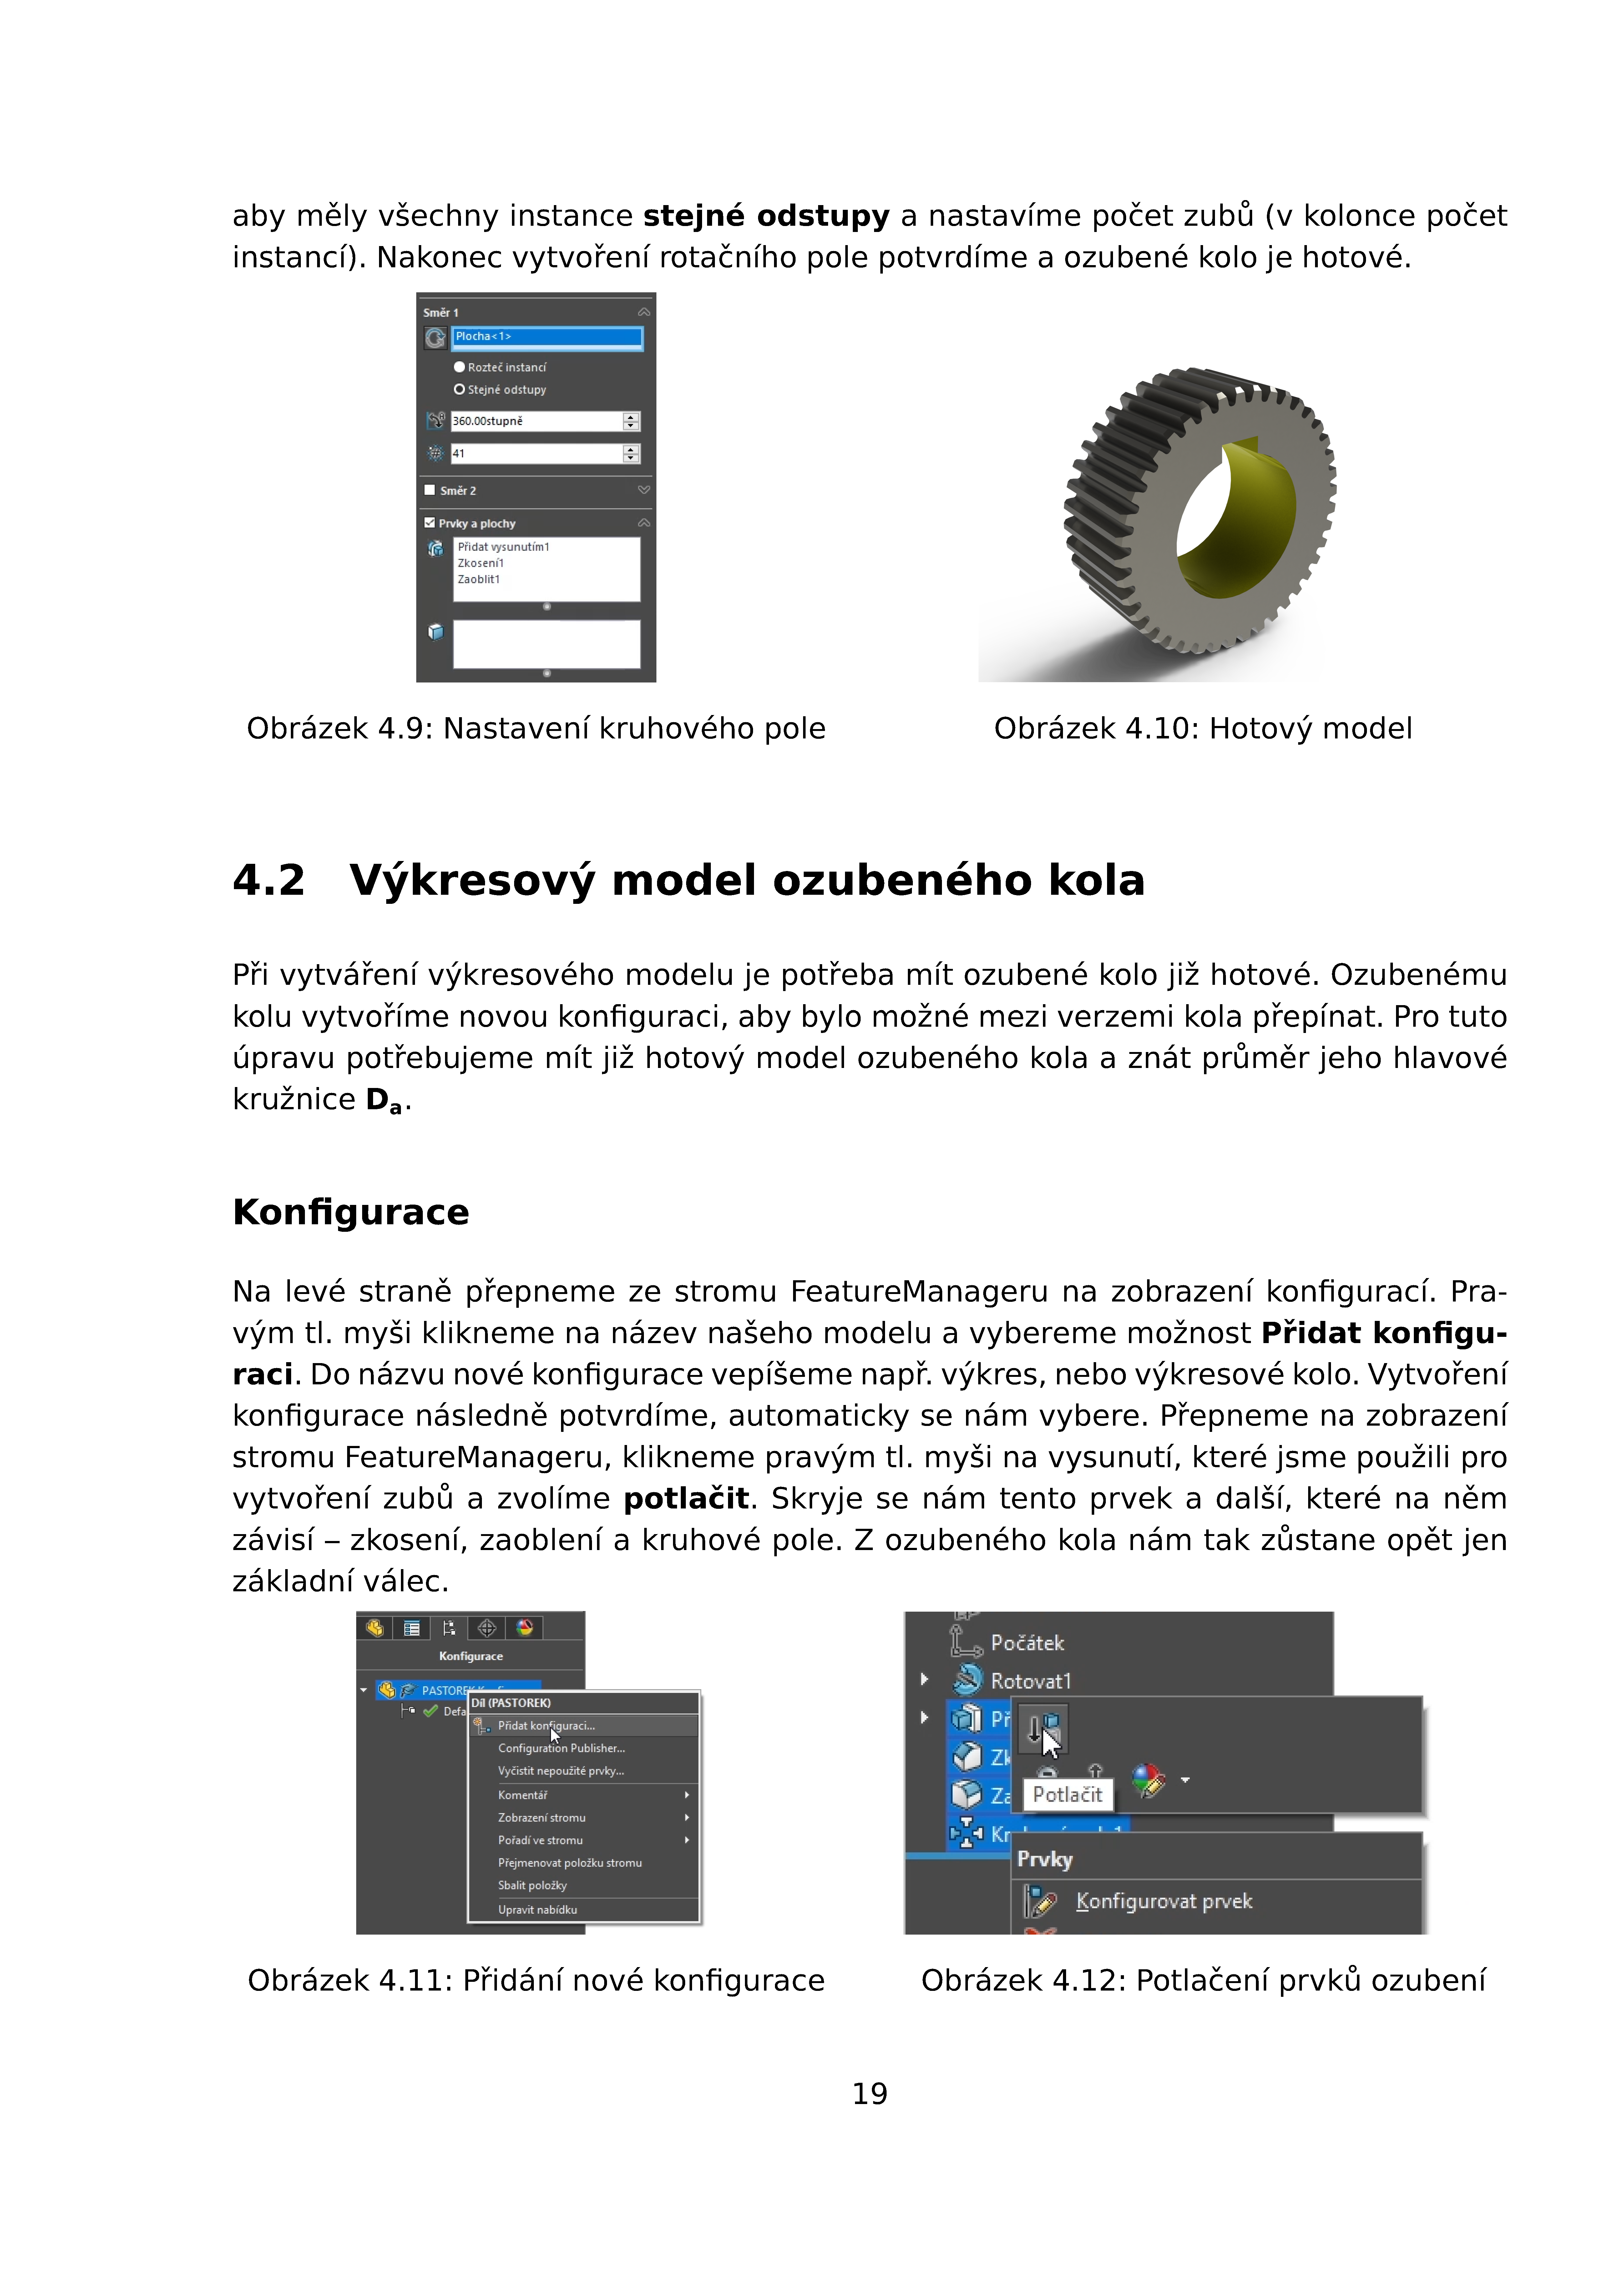
\includegraphics[width=0.8\textwidth]{img/020/guide2.png}
        \caption{Tištěné materiály}
        \label{fig:thumb4}
    \end{minipage}
\end{figure}


\subsection{Otázky a úkoly}
Na konci každého návodu jsou umístěny doplňující otázky a úkoly, které studentům umožňují si procvičit postupy, nebo ověřit získané znalosti.
Řešení těchto otázek a úkolů jsou záměrně umístěny v sekci pro vyučující, která tvoří přílohu těchto tištěných materiálů.

\subsection{Dostupnost tisknutelných materiálů}
Verze bez metodických pokynů a řešení úloh jsou (\fxnote[inline=true]{\textcolor{red}{BUDOU}}) volně k dispozici na webu \href{https://www.p3dportal.cz}{www.p3dportal.cz} v sekci \enquote{Ke stažení}.
O variantu pro vyučující je možné si zažádat na e-mailové adrese \href{mailto:info@parallaxproduction.cz}{info@parallaxproduction.cz}.

\section{Výukový portál P3D}


\section{Doplňující }

